\documentclass[a4paper,12pt]{article}
\usepackage[utf8]{inputenc}
\usepackage{geometry}
\usepackage{amsmath}
\geometry{margin=1in}
\usepackage{listings}
\usepackage{xcolor}
\usepackage{pgf-umlcd}

\lstset{
    basicstyle=\ttfamily\small,
    keywordstyle=\color{blue}\bfseries,
    stringstyle=\color{red},
    commentstyle=\color{green!50!black},
    numbers=left,
    numberstyle=\tiny,
    stepnumber=1,
    numbersep=5pt,
    breaklines=true,
    frame=single,
    tabsize=2,
    showspaces=false,
    showstringspaces=false
}

\title{Arbitrary Precision Arithmetic Library: Implementation Overview}
\author{Harikrishna S - CS24BTECH11030}
\date{May 2025}

\begin{document}

\maketitle

\section{Introduction}
This report describes the implementation of a Java-based Arbitrary Precision Arithmetic Library, designed to perform high-precision integer and floating-point arithmetic. The library `arbritaryarithmetic` includes three core classes: \texttt{AInteger}, \texttt{AFloat}, and \texttt{ANumber}, with a focus on efficient storage and arithmetic operations.

\section{Class Structure and Data Representation}

\subsection{ANumber}
The abstract base class \texttt{ANumber} defines common properties for \texttt{AInteger} and \texttt{AFloat}. It includes:
\begin{itemize}
    \item \texttt{num\_list}: An \texttt{ArrayList<Integer>} storing digits of the number.
    \item A \texttt{ZeroDivisionError} exception for handling division by zero.
\end{itemize}

\subsection{AInteger}
The \texttt{AInteger} class handles arbitrary-precision integer arithmetic. Each digit is stored in \texttt{num\_list}, where:
\begin{itemize}
    \item Index 0 represents the units place, index 1 the tens place, and so on.
    \item Negative numbers are represented by storing negative digits in \texttt{num\_list} (e.g., -123 is stored as [-3, -2, -1]).
\end{itemize}

\subsection{AFloat}
The \texttt{AFloat} class extends \texttt{ANumber} for floating-point arithmetic. It uses:
\begin{itemize}
    \item \texttt{num\_list} for digits, similar to \texttt{AInteger}.
    \item A \texttt{power} property, where the floating-point value is computed as $\text{num\_list} \times 10^{\text{power}}$.
    \item Negative numbers are represented with negative digits in \texttt{num\_list}.
\end{itemize}

\section{Arithmetic Operations}

\subsection{Addition and Subtraction}
For \texttt{AInteger}:
\begin{itemize}
    \item Digits at corresponding indices are added or subtracted.
    \item A separate \texttt{resolve} function handles carry-over, normalizing the result by propagating carries or borrows.
\end{itemize}
For \texttt{AFloat}:
\begin{itemize}
    \item Operands are aligned to the same \texttt{power} by shifting digits.
    \item Addition or subtraction is then performed as in \texttt{AInteger}, followed by carry resolution.
\end{itemize}

\subsection{Multiplication and Division}
Both classes implement multiplication and division mimicking manual arithmetic:
\begin{itemize}
    \item \textbf{Multiplication}: Each digit of one operand is multiplied by the entire second operand, with appropriate shifts (e.g., appending zeros for place values). Results are summed.
    \item \textbf{Division}: Uses a long division approach, iteratively subtracting multiples of the divisor from the dividend.
\end{itemize}

\subsection{Helper Functions}
Supporting operations include:
\begin{itemize}
    \item \texttt{\_left\_shift} and \texttt{\_right\_shift}: Adjust the position of digits in \texttt{num\_list}.
    \item \texttt{\_negate}: Inverts the sign of the number by negating each digit.
    \item \texttt{\_is\_negative}: Checks if the number is negative based on \texttt{num\_list} values.
\end{itemize}

\subsection{Design diagram}
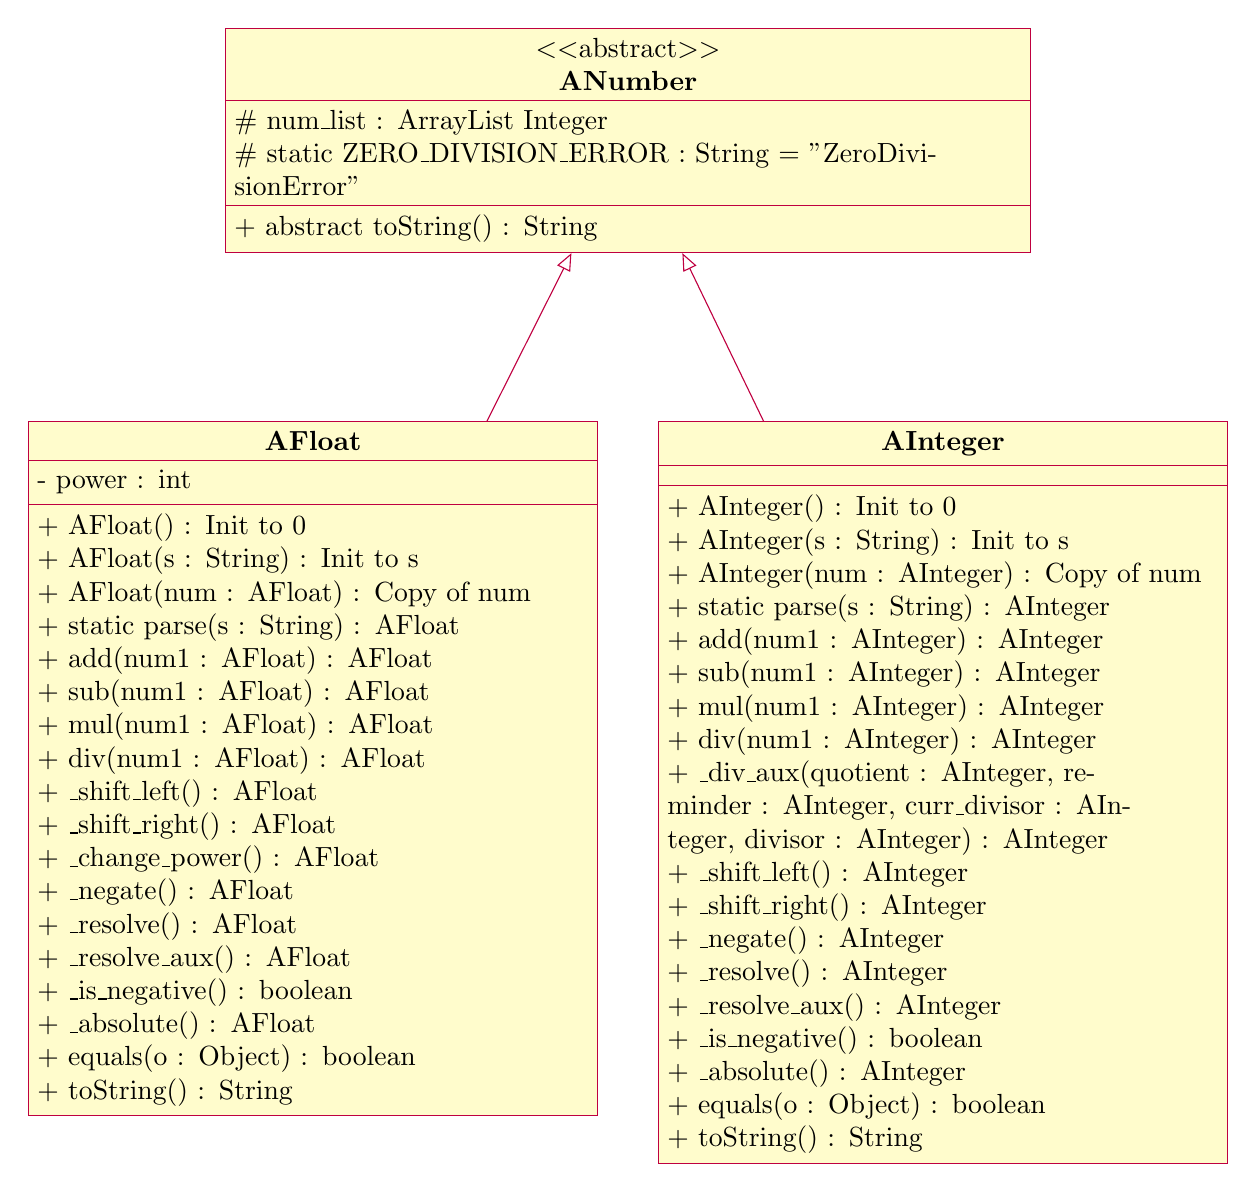
\begin{tikzpicture}
    \begin{abstractclass}[text width=10cm]{ANumber}{0,1}
        \attribute{\# num\_list : ArrayList Integer}
        \attribute{\# static ZERO\_DIVISION\_ERROR : String = "ZeroDivisionError"}

        \operation{+ abstract toString() : String }
    \end{abstractclass}

    \begin{class}[text width=7cm]{AFloat}{-4,-4}
        \inherit{ANumber}
        \attribute{- power : int}
        
        \operation{+ AFloat() : Init to 0}
        \operation{+ AFloat(s : String) : Init to s}
        \operation{+ AFloat(num : AFloat) : Copy of num}
        \operation{+ static parse(s : String) : AFloat}
        
        \operation{+ add(num1 : AFloat) : AFloat}
        \operation{+ sub(num1 : AFloat) : AFloat}
        \operation{+ mul(num1 : AFloat) : AFloat}
        \operation{+ div(num1 : AFloat) : AFloat}
        \operation{+ \_shift\_left() : AFloat}
        \operation{+ \_shift\_right() : AFloat}
        \operation{+ \_change\_power() : AFloat}
        \operation{+ \_negate() : AFloat} 
        \operation{+ \_resolve() : AFloat}
        \operation{+ \_resolve\_aux() : AFloat}
        \operation{+ \_is\_negative() : boolean}
        \operation{+ \_absolute() : AFloat}
        \operation{+ equals(o : Object) : boolean}
        \operation{+ toString() : String}
    \end{class}

    \begin{class}[text width=7cm]{AInteger}{4,-4}
        \inherit{ANumber}
        \operation{+ AInteger() : Init to 0}
        \operation{+ AInteger(s : String) : Init to s}
        \operation{+ AInteger(num : AInteger) : Copy of num}
        \operation{+ static parse(s : String) : AInteger}
        
        \operation{+ add(num1 : AInteger) : AInteger}
        \operation{+ sub(num1 : AInteger) : AInteger}
        \operation{+ mul(num1 : AInteger) : AInteger}
        \operation{+ div(num1 : AInteger) : AInteger}
        \operation{+ \_div\_aux(quotient : AInteger, reminder : AInteger, curr\_divisor : AInteger, divisor : AInteger) : AInteger}
        \operation{+ \_shift\_left() : AInteger}
        \operation{+ \_shift\_right() : AInteger}
        \operation{+ \_negate() : AInteger} 
        \operation{+ \_resolve() : AInteger}
        \operation{+ \_resolve\_aux() : AInteger}
        \operation{+ \_is\_negative() : boolean}
        \operation{+ \_absolute() : AInteger}
        \operation{+ equals(o : Object) : boolean}
        \operation{+ toString() : String}
    \end{class}
\end{tikzpicture}

\section{Limitations and Potential Improvements}
\begin{itemize}
    \item The separate carry-over mechanism in \texttt{resolve} could be integrated into a single loop for efficiency.
    \item Multiplication performance for large numbers could be improved by memoizing intermediate results.
\end{itemize}

\end{document}